\documentclass{article}

% The preceding line is only needed to identify funding in the first footnote. If that is unneeded, please comment it out.
\usepackage{cite}
\usepackage{amsmath,amssymb,amsfonts}
\usepackage{algorithmic}
\usepackage{graphicx}
\usepackage{float}
\usepackage{textcomp}
\usepackage{xcolor}
\usepackage{outlines}
\usepackage{enumitem}
\setenumerate[1]{label=\arabic*.}
\setenumerate[2]{label=\alph*.}

\def\BibTeX{{\rm B\kern-.05em{\sc i\kern-.025em b}\kern-.08em
    T\kern-.1667em\lower.7ex\hbox{E}\kern-.125emX}}
\begin{document}
\begin{titlepage}
    \begin{center}
        \vspace{4cm}
        \large
        \textbf{
            Progress Report III \\
            Dylan Miracle \\
            ICS 698-02 \\
            Spring 2021 \\
            Mar 2, 2021 \\
            Dr. Jigang Liu
        }
    \end{center}
\end{titlepage}
\title{Getting started coding quantum computers with QASM and Qiskit}

\author{Dylan Miracle\\
\textit{Department of Computer Science} \\
\textit{Metropolitan State University}\\
St. Paul, Minnesota, USA \\
dylan.miracle@my.metrostate.edu
}

\maketitle

\tableofcontents

\section{Preliminary findings}
Quantum computing has a rich theoretical background but practical quantum computers have only recently become available to researchers and business users. These computers are still rare and operated by a small number of hardware vendors. The dominant paradigm for programing quantum computers is the gate model of quantum computing that defines a sequence of operations on a set of qubits. In this paper we introduce a fundamental quantum circuit and demonstrate its implementation using an intermediate representation, QASM, and a higher level quantum computing framework Qiskit. 

While QASM and Qiskit are specific to IBM, the model they use of intermediate representation and higher level language is present with other vendors (see Rigetti) and a good way to understand and control a quantum computer. An intermediate language gives us a method to write out specific gates used in most quantum computing algorithms, while the higher level framework lets us use standard computing. 

Specifically we will use the example of the Bell states. These are the most basic states that exhibit the main features of quantum computing, namely superposition and entanglement of qubits. The development of this basic quantum circuit will take the following approach:
\begin{outline}[enumerate]
\1 Qubits -- fundamental unit of quantum computing. Two element vector with a complex number amplitude for each computational basis 1 or 0. Measured as either 1 or 0
\1 Bell state - 
    \2 Hadamard gate - show the matrix multiplication that takes a single qubit and puts it into superposition
    \2 CNOT gate -- show the matrix multiplication that takes the superposed qubit and another 0 qubit and entangles them
\1 The circuit diagram for this set of operations. See below.
\1 QASM bell state example
\1 Qiskit bell state example
\end{outline}
\section{Tables/figures/charts}
\subsection{Circuit diagram}
This diagram shows the standard circuit representation for gate model quantum computing. This is a simple circuit that creates a Bell state with two starting qubits, then shows the measurements of those qubits being written into classical bits.
\begin{figure}[H]
    \centering
    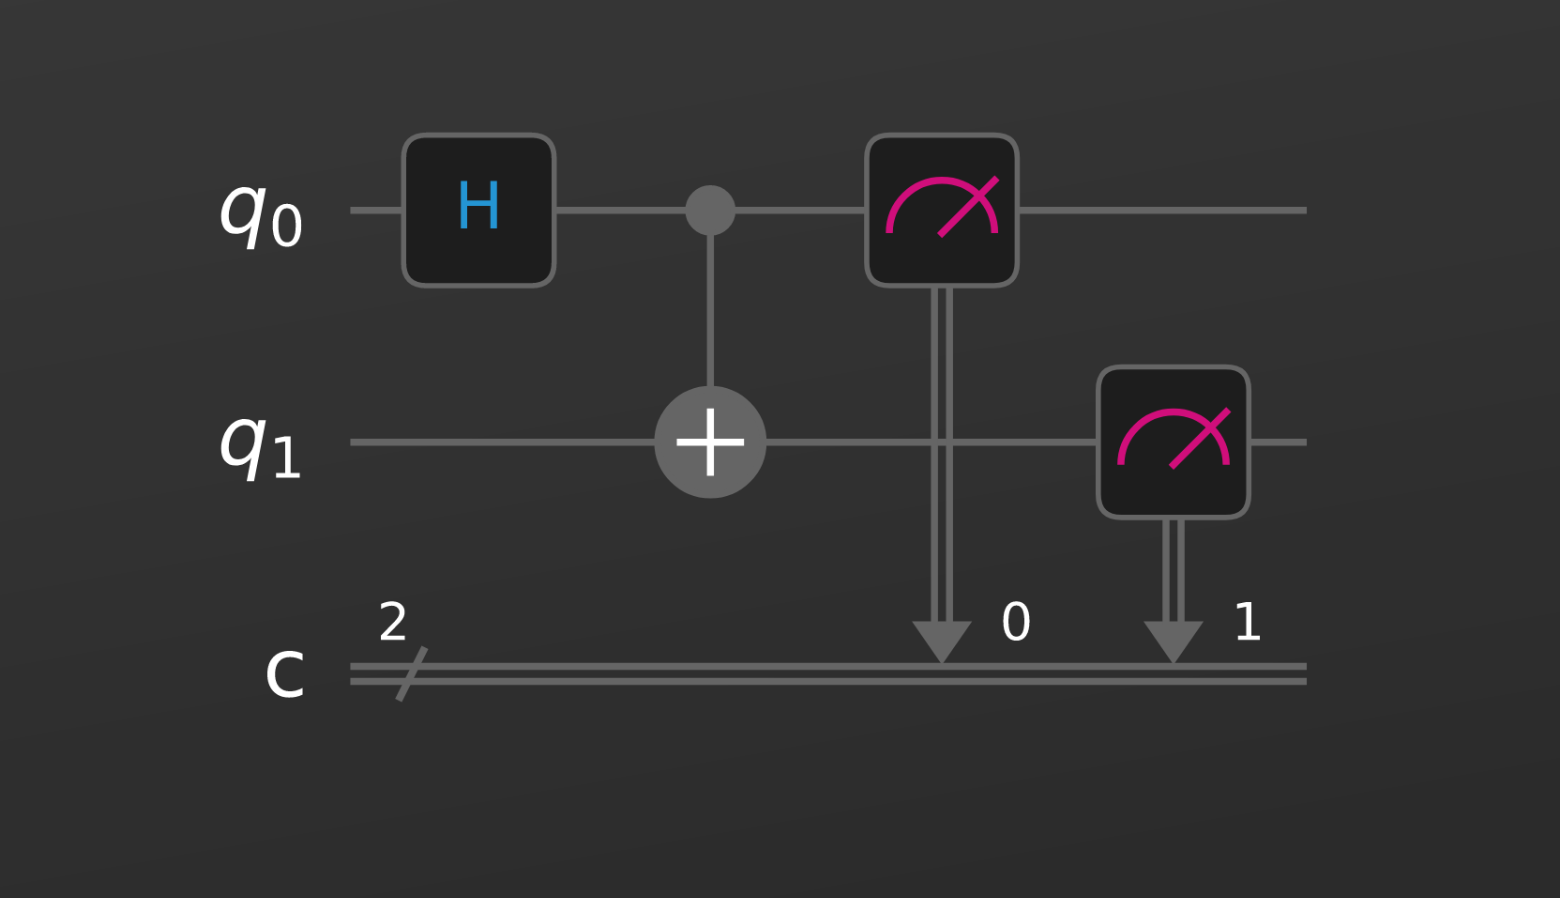
\includegraphics[width=0.75\textwidth]{circuit.png}
    \caption{A quantum circuit that will create a Bell state with two qubits.}
\end{figure}

\subsection{Quantum development flowchart}
Developing quantum algorithms is found to follow a flow from the quantum mechanics, to a quantum circuit, to intermediate representations, to higher level frameworks. This flow illustrates the findings of this paper and will serve as an outline for our exploration of quantum computing. 
\begin{figure}[H]
    \centering
    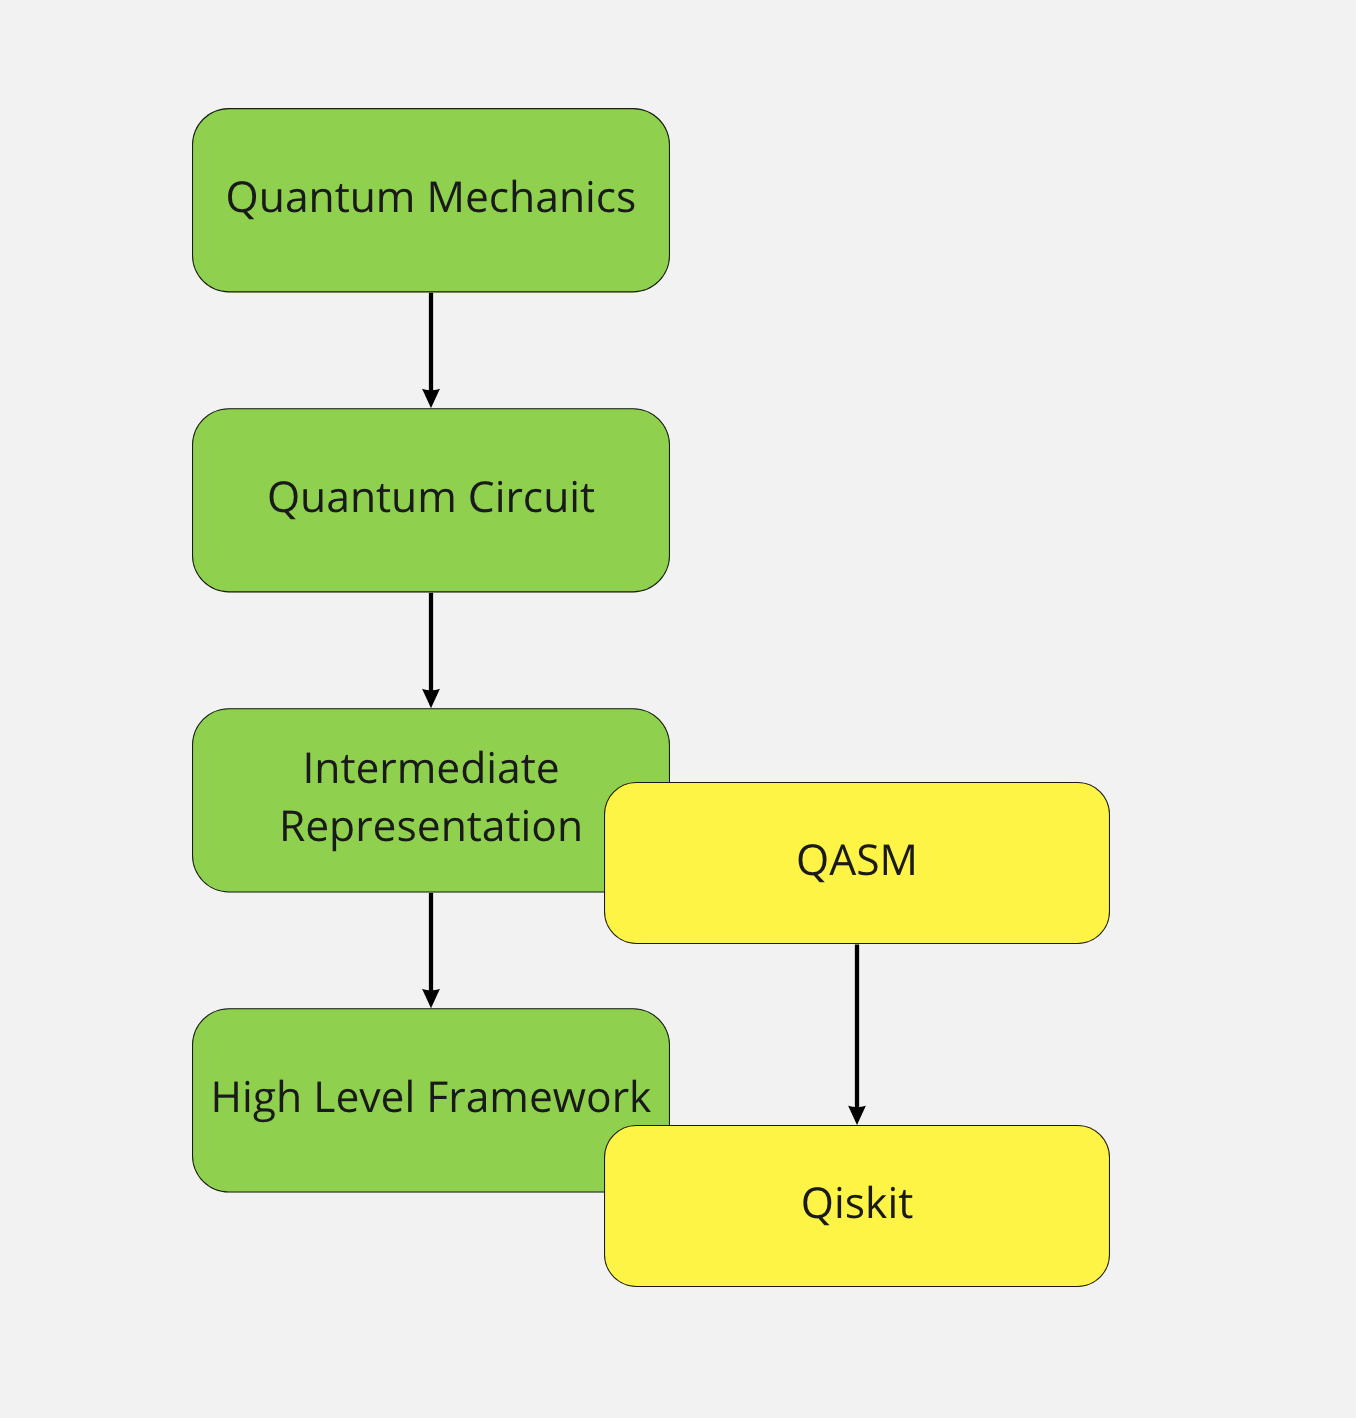
\includegraphics[width=0.75\textwidth]{flowchart.png}
    \caption{The quantum development flow.}
\end{figure}

\section{Preliminary conclusion}
Developers can write code for quantum computers by learning frameworks in already existing languages. Several frameworks studied in the literature review have python frameworks. Python is often used because it is broadly adopted by the scientific community and creates a lower barrier to entry than some other languages might. For example Microsoft's Q\# language uses a combination of F\# and C\# that is less familiar to people not used to writing code in both of those languages. A good framework gives developers access to the tools needed to run quantum gates, but also standard computing tools that are helpful in interpreting results. The model used by qiskit to run jobs and return results means that programmers can predict what kind of data they will be dealing with before they fully understand the algorithms being used on the quantum side. As more software has a quantum components having well defined result data and job definitions means that software developers can create code for interpreting results and dealing with the output of quantum computers without becoming quantum computing experts.

Quantum computing will not stand on its own, but will always be employed in tandem with classical computing. This is as simple as using standard computers to create flow control or as advanced as using the fully featured APIs needed to connect to actual quantum hardware. As discussed the data returned by quantum algorithms will be interpreted and represented by classical computers. It is possible to currently develop software that will use quantum results in the future because well designed frameworks like qiskit have a standard workflow and results data structure.


\section{Two arguments or reasons differentiating results}
Much work has been done to develop quantum computing frameworks. These frameworks are racing to increase functionality and capabilities for advanced users. This paper should give an overview of some of the fundamentals of quantum computing for an advanced undergraduate or software developer without a background in quantum mechanics. The audience for most quantum computing work is physics PhDs making it inaccessible to a typical software developer. This has a chilling effect on a bourgeoning industry. When we think about the great contributions to our modern information age we often end up thinking about hackers in a garage just as much as engineers in a clean room. The target audience of this paper differentiates it from the existing literature. 

This work gives an overview, from mathematical development of a simple quantum circuit to implementation with a high level quantum framework. Readers will get a taste of the complete quantum pipeline. This is valuable because much work focuses on one area of the ecosystem instead of walking those new to quantum mechanics through the complete process of how to implement some quantum code. For example, there are many papers detailing the use of a particular language, or that go into depth on specific quantum algorithms. Even though we focus on a specific framework the model of understanding quantum development proposed by this paper will be useful to anyone who wants to delve further into quantum computing. 



\section{Two facts showing work is non-trivial}

In the early days of digital computing a programmer needed a deep understanding of electrical engineering to program computers. The programming was low level involving digital logic gates and binary code. Abstractions were slowly built in to allow programmers to manipulate abstract data types so that now you can prgram a computer in a human readable language that uses high level concepts such as object inheritance and lambda calculus. Quantum computing is in its early phase and will likely progress to human human readable abstractions quickly. Developers who want to learn to program quantum computers will be served well to learn a programming framework to experiment with as opposed to taking a PhD in physics before learning the basics of quantum computing. It is not necessary to understand how a computer stores a string to build a web page, we should expect the same kinds of abstractions from quantum computing in the coming decade.

Frameworks such as qiskit and others already give a programmer access to many tools for interpreting and experimenting with quantum computers. This work aims to show an interested developer how to get started programming and interpreting quantum results. After reading this paper, for example, a developer would be able to create a webpage to display quantum results because they could understand how the result data is returned. Without needing to know the ins-and-outs of quantum computing they would be able to manipulate result data with a classical computer. This is a valuable tool because quantum computers will always be used with classical computers.

\end{document}
